\section{Prerequisites}
\subsection{Axial Algebras}
Axial algebras have been defined in multiple papers so this section will be brief. For an in-depth discussion, we recommend to look at \cite{hall2015universal}, \cite{khasraw2020structure} and \cite{mcinroy2022axial}. A starting point is the definition of a fusion law in \cite{de2020decomposition}. 
\begin{defn}
Let $\mcal{F}$ be a set and let $\star: \mcal{F} \times \mcal{F} \rightarrow 2^{\mcal{F}}$ be a binary operator, where $2^{\mcal{F}}$ denotes the power set of $\mcal{F}$. We call the pair $\fustar{F}$ a \emph{fusion law}. We say it is  \emph{symmetric} if for all $x,y\in \mcal{F}$, we have $x\star y=y\star x$.  
\end{defn}
\begin{note}
When a fusion law $\fustar{F}$ is clear, we will refer to it by $\mcal{F}$. 
\end{note}
For axial algebras, as they are commutative, fusion laws are considered to be symmetric. Given a fusion law, one is able to grade it using a group. We will denote the group operation by juxtaposition. 
\begin{defn} Let $\fustar{F}$ be a fusion law and $T$ be a group. We say $\mcal{F}$ is $T$-graded if there exists a map $\xi: \mcal{F}\rightarrow T$
such that for all $\lm, \mu\in \mcal{F}$,
$$\xi(\nu)=\xi(\lm)\xi(\mu)$$
for all $\nu\in \lm\star \mu$.
\end{defn}
\begin{table}[b]
\begin{minipage}{.5\linewidth}
\centering
\begin{tabular}{|c|c|c|c|} 
 \hline
  $\star$& 0 & 1 & $\eta$\\ [0.4ex] 
 \hline
 0 & 0 &  & $\eta$\\ 
 \hline
 1 &  & 1 & $\eta$\\
 \hline
 $\eta$ & $\eta$ & $\eta$& 1, 0\\
 \hline
\end{tabular}
\caption{Fusion law of $\jor{\eta}$}\label{J Table}
\end{minipage}%
\begin{minipage}{.5\linewidth}
\centering
\begin{tabular}{|c|c|c|c|c|} 
 \hline
  $\star$& 0 & 1 & $\alpha$ & $\beta$\\ [0.4ex] 
 \hline
 0 & 0 &  & $\alpha$ & $\beta$\\ 
 \hline
 1 &  & 1 & $\alpha$ & $\beta$\\
 \hline
 $\alpha$ & $\alpha$ & $\alpha$& 1, 0 & $\beta$\\
 \hline
 $\beta$ & $\beta$ & $\beta$ & $\beta$ & 1, 0, $\alpha$\\
 \hline
 \end{tabular}
 \caption{Fusion law of $\mon{\al,\bt}$}
 \label{M Table}
 \end{minipage}
\end{table}
The fusion laws that are used in this paper are $\jor{\eta}$ and $\mon{\al,\bt}$, which are defined in Tables \ref{J Table} and \ref{M Table} respectively. Let $C_2=\{e,s\}$ be the cyclic group of order two, where $e$ is the identity element. Then $\jor{\eta}$ and $\mon{\al,\bt}$ are both $C_2$-graded where $0$, $1$, $\al$ are mapped to $e$ and $\eta$, $\bt$ are mapped to $s$.

Let $A$ be a commutative algebra over $\F$. For $a\in A$, the adjoint map of $a$ is $\text{ad}_a: A \rightarrow A$ with $\text{ad}_a(x)=ax$ for all $x\in A$. Let $\text{Spec}(a)$ be the set of eigenvalues of $\text{ad}_a$ and for $\lambda \in \F$, let $A_{\lambda}(a)$ be the $\lambda$-eigenspace of $\text{ad}_a$. Note that $A_\lambda(a)$ is non-trivial if and only if $\lambda \in \spec{a}$. For $S\subseteq \F$, we write $A_S(a) := \oplus_{\lm \in S} A_\lm(a)$.
We will use the definition of axes and axial algebras in \cite{khasraw2020structure}. 
\begin{defn}
Let $\fustar{F}$ be a fusion law, $A$ be a commutative algebra over $\F$, and $a\in A$. We have that $a$ is a (primitive) $\mcal{F}$-\emph{axis} if it satisfies the following:
\begin{enumerate}
    \item[A$1.$] $a$ is an idempotent; $a^2=a$,
    \item[A$2.$] $a$ is semisimple and $\spec{a}\subseteq \mcal{F}$; that is, $A=A_\mcal{F}(a)$,
    \item[A$3$.] For all $\lm,\mu \in \mcal{F}$, $A_\lm(a)A_\mu(a) \subseteq A_{\lm \star \mu}(a)$, and 
    \item[A$4$.] $A_1(a)=\GenG{a}$.
\end{enumerate}
We call an $\mcal{F}$-axis non-primitive if it satisfies A$1$-A$3$ and not A$4$. 
\end{defn}
\begin{defn}
Let $\fustar{F}$ be a fusion law, $A$ be a commutative algebra over $\F$, and $X$ be a set of (primitive) $\mcal{F}$-axes in $A$. We call $(A,X)$ a (primitive) $\mcal{F}$-\emph{axial algebra} if $X$ generates $A$.
\end{defn}
\begin{no}
When $X$ and $\mcal{F}$ are clear, we will refer to the axial algebra by $A$. As this paper is concerned with only $2$-generated algebras, we will assume $|X|=2$. We will assume all axial algebras and axes to be primitive. If that is not the case, we will explicitly say when an axis or an axial algebra is not.  
\end{no}
\begin{defn}\label{Proj}
    Let $(A,X)$ be a $\mcal{F}$-axial algebra and let $a$ be a $\mcal{F}$-axis. For any $v\in A$, $v=\lm_a(v) a + \sum_{\gm \in \mcal{F}\backslash\{1\}} v_\gm$ where $v_\gm \in A_\gm(a)$ due to A$2$. Let
    \begin{eqnarray*}
        \lm_a : A &\rightarrow& \F\\
 v &\mapsto& \lm_a(v).      
    \end{eqnarray*}
    We call this map the \emph{projection map} of $a$. This is a well-defined $\F$-linear map from Proposition 2.4 in \cite{franchi20211}.
\end{defn}
\begin{defn}
Let $\F$ have characteristic not equal to $2$. Suppose $\fustar{F}$ is a $C_2$-graded fusion law with morphism $\xi$, and $(A,X)$ is a $\mcal{F}$-axial algebra. Suppose $a$ is a $\mcal{F}$-axis in $A$ and let $\tu{a}:A\rightarrow A$. For $v\in A_\lm(a)$, we define $\tu{a}$ to be the following 
\begin{eqnarray*}
        \tau_a(v)=
        \begin{cases}
            v & \text{if } \xi(\lm)=e\\
            -v & \text{if } \xi(\lm)=s
        \end{cases}
    \end{eqnarray*}
By A$2$, this definition of $\tu{a}$ extends to the entire algebra and it can be shown to an automorphism of $A$. We call $\tu{a}$ the \emph{Miyamoto involution} of $a$.
\end{defn}
\begin{exmp}
For $(A,X)$ a $\jor{\eta}$-axial algebra and $\jor{\eta}$-axis $a$, $\tu{a}$ acts as the identity map on $A_{\{0,1\}}(a)$ and negative identity map on $A_\eta(a)$.

Similarly for $(A,X)$ a $\mon{\al,\bt}$-axial algebra and $\mon{\al,\bt}$-axis $a$, $\tu{a}$ acts as the identity map on $A_{\{0,1,\al\}}(a)$ and negative identity map on $A_\bt(a)$.
\end{exmp}


\begin{defn}
We call a fusion law, $\fustar{F}$, \emph{Seress} if:
\begin{enumerate}
    \item $0 \in \mcal{F}$, and
    \item $\lambda \star 0 = \{\lambda\}$ for $\lambda \neq 1$, and $1\star 0 = \emptyset$.
\end{enumerate}
\end{defn}
\begin{exmp}
Both $\jor{\eta}$ and $\mon{\al,\bt}$ are Seress.
\end{exmp}
The following result was proven in \cite{hall2015universal}. Seress originally proved it for fusion law $\mon{\frac{1}{4},\frac{1}{32}}$ but has now been generalised to all fusion laws that are Seress. 
\begin{lem}[Seress Lemma]\label{Seress}
Let $\fustar{F}$ be Seress and $(A,X)$ be an $\mcal{F}$-axial algebra. Then every $\mcal{F}$-axis $a\in A$ associates with $A_{\{0,1\}}(a)$. That is, for $x\in A$ and $u\in A_{\{0,1\}}(a)$, we have
\[ a(xu)=(ax)u.\]
\end{lem}
This result will be useful when finding the GAP equations in the appendix.
\subsection{Axets}
The idea of axets can be traced back to \cite{mcinroy2020expansion}, where M\textsuperscript{c}Inroy and Shpectorov looked at shapes of an algebra for their algorithm. Later in \cite{mcinroy2021forbidden}, they defined axets and stated results around them. We recommend that the reader looks at \cite[Section 3]{mcinroy2021forbidden} and \cite[Section 6.3]{mcinroy2022axial} for a greater introduction.
\begin{defn}
Let $S$, $G$ be groups and $G$ acts on a set $X$. Suppose there is a map $\tau:X\times S \rightarrow G$, denoted $\tau(x,s)=\tu{x}(s)$. Then $(G,X,\tau)$ is called an $S$-axet if for all $x\in X$, $s,s'\in S$ and $g\in G$, the following properties hold:
\begin{enumerate}
    \item $\tu{x}(s)\in G_x$;
    \item $\tu{x}(ss')=\tu{x}(s)\tu{x}(s')$; and 
    \item $\tu{xg}(s)=\tu{x}(s)^g$.
\end{enumerate}
If $S$, $G$ and $\tau$ are clear, we denote the axet by $X$.
For each $x\in X$, let $T_x:=\text{Im}(\tu{x})$, which is called the axial subgroup corresponding to $x$.
\end{defn}
\begin{rem}
The first two points makes $\tau_x$ a group homomorphism between $S$ and $G_x$ for all $x\in X$. One can show that for all $x\in X$, $T_x\subseteq Z(G_x)$ and $[S,S]\subseteq \text{ker}(\tu{x})$. Hence we can assume $S$ to be abelian.   
\end{rem}

\begin{defn}
Let $(G,X,\tau)$ be an $S$-axet and $Y\subseteq X$. Then $Y$ is \emph{closed} if $Y$ is invariant under $T_y$ for all $y\in Y$. For $Z\subseteq X$, the \emph{closure} of $Z$ in $X$ is the smallest closed subset containing $Z$, denoted by $\GenG{Z}$. We say that $\GenG{Z}$ is $k$-\emph{generated} if there exist $x_1,...,x_k\in X$ such that $\GenG{Z}=\GenG{x_1,...,x_k}$.
\end{defn}
\begin{exmp}
Let $(A,X)$ be an $\mcal{F}$-axial algebra where $\mcal{F}$ is $C_2$-graded. Take $\tilde{X}$ to be the set of all $\mcal{F}$-axes in $A$ and $G=\text{Aut}(A)$. For $x\in \tilde{X}$, let $\tu{e}(x)$ to be the identity map and $\tu{s}(x)$ to be the Miyamoto involution of $x$. Then $(G,\tilde{X},\tau)$ is a $C_2$-axet.

Let $Y=\GenG{X}$, $H=G_Y$ and $\tau'$ be the restriction of $\tau$ to the domain $Y\times C_2$. Then $(H,Y,\tau')$ is $C_2$-axet. Suppose that $|X|=2$ whence $(H,Y,\tau')$ is a $2$-generated axet and this paper will solely be looking at these.
\end{exmp}
We will now discuss some $2$-generated $C_2$-axets. 
\begin{exmp}
The following are in Examples 3.22 and 3.25 in \cite{mcinroy2021forbidden}.
\begin{enumerate}
    \item For $n\geq 2$, denote $X(n)$ to be the vertices of a regular $n$-gon. Let $X=X(n)$ and $a$, $b$ be adjacent vertices in $X$. We have that $G=D_{2n}$ and for $a\in X$, $\tu{a}(e)$ is the identity map and $\tu{a}(s)$ is the reflection of $X$ at vertex $a$. 
    \item Let $X=X(\infty)\cong\Z$ and $a$, $b$ be adjacent points on $X$. Then $G=D_\infty$ and for $a\in X$, $\tu{a}(e)$ is the identity map and $\tu{a}(s)$ is the reflection of $X$ at point $a$.
    \item Let $n=4k$ and we look at the $C_2$-axet $(D_{8k}, X(4k), \tau)$. We now identify opposite vertices of one bipartite half of the polygon denoting this by $X':=X'(k+2k)$. Let $G=D_{4k}$ and $\tau'$ to be the restriction of the domain to $X'\times C_2$. This is also an $C_2$-axet and we call $X'$ \emph{skew}. 
\end{enumerate}
\end{exmp}
We will now state Theorem 3.27 in \cite{mcinroy2021forbidden}.
\begin{prop}\label{axet thm}
Let $X=\GenG{a,b}$ be a $2$-generated $C_2$-axet with $n$ axes, where $n\geq 2$ and $n=\infty$. Then $X$ is isomorphic to 
\begin{enumerate}
    \item[$1.$] $X(n)$, or
    \item[$2.$] $X'(k+2k)$, where $k\in \N$ and $n=3k$.
\end{enumerate}
\end{prop}
In Figures \ref{Skew-1} and \ref{Skew-2}, we show $X'(1+2)$ and $X'(2+4)$, where the dotted arrow represents equivalence between two vertices. From now on, we will be working with $X'(1+2)$ however we will talk about more general skew axets in the final section. 

\begin{figure}[ht]
\centering
\begin{minipage}{.5\textwidth}
\centering
\tikzset{every picture/.style={line width=0.75pt}} %set default line width to 0.75pt        

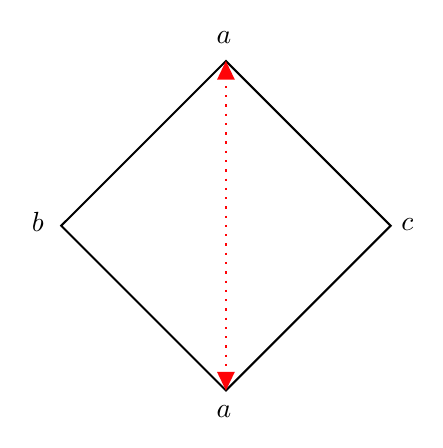
\begin{tikzpicture}[x=0.75pt,y=0.75pt,yscale=-1,xscale=1]
%uncomment if require: \path (0,300); %set diagram left start at 0, and has height of 300

%Shape: Rectangle [id:dp9553545350293062] 
\draw   (307.01,75.59) -- (386.35,154.93) -- (307.01,234.28) -- (227.66,154.93) -- cycle ;
%Straight Lines [id:da4973981194045116] 
\draw [color={rgb, 255:red, 255; green, 4; blue, 8 }  ,draw opacity=1 ] [dash pattern={on 0.84pt off 2.51pt}]  (307.01,78.59) -- (307.01,231.28) ;
\draw [shift={(307.01,234.28)}, rotate = 270] [fill={rgb, 255:red, 255; green, 4; blue, 8 }  ,fill opacity=1 ][line width=0.08]  [draw opacity=0] (8.93,-4.29) -- (0,0) -- (8.93,4.29) -- cycle    ;
\draw [shift={(307.01,75.59)}, rotate = 90] [fill={rgb, 255:red, 255; green, 4; blue, 8 }  ,fill opacity=1 ][line width=0.08]  [draw opacity=0] (8.93,-4.29) -- (0,0) -- (8.93,4.29) -- cycle    ;

% Text Node
\draw (301,60) node [anchor=north west][inner sep=0.75pt]   [align=left] {$\displaystyle a$};
% Text Node
\draw (212,147) node [anchor=north west][inner sep=0.75pt]   [align=left] {$\displaystyle b$};
% Text Node
\draw (301,240) node [anchor=north west][inner sep=0.75pt]   [align=left] {$\displaystyle a$};
% Text Node
\draw (390,150) node [anchor=north west][inner sep=0.75pt]   [align=left] {$\displaystyle c$};
\end{tikzpicture}
\caption{$X'(1+2)$}
\label{Skew-1}
\end{minipage}%
\begin{minipage}{.5\textwidth}
\centering
\tikzset{every picture/.style={line width=0.75pt}} %set default line width to 0.75pt        

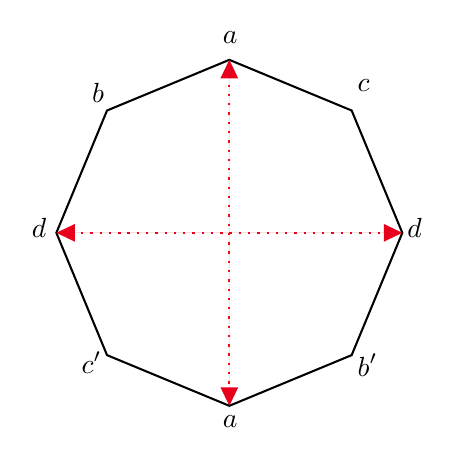
\begin{tikzpicture}[x=0.75pt,y=0.75pt,yscale=-1,xscale=1]
%uncomment if require: \path (0,300); %set diagram left start at 0, and has height of 300

%Shape: Regular Polygon [id:dp8058063624355654] 
\draw   (408,138.34) -- (383.59,197.27) -- (324.66,221.68) -- (265.73,197.27) -- (241.32,138.34) -- (265.73,79.41) -- (324.66,55) -- (383.59,79.41) -- cycle ;
%Straight Lines [id:da4976793908038122] 
\draw [color={rgb, 255:red, 255; green, 4; blue, 8 }  ,draw opacity=1 ][fill={rgb, 255:red, 240; green, 0; blue, 28 }  ,fill opacity=1 ] [dash pattern={on 0.84pt off 2.51pt}]  (324.66,58) -- (324.66,218.68) ;
\draw [shift={(324.66,221.68)}, rotate = 270] [fill={rgb, 255:red, 232; green, 1; blue, 29 }  ,fill opacity=1 ][line width=0.08]  [draw opacity=0] (8.93,-4.29) -- (0,0) -- (8.93,4.29) -- cycle    ;
\draw [shift={(324.66,55)}, rotate = 90] [fill={rgb, 255:red, 232; green, 1; blue, 29 }  ,fill opacity=1 ][line width=0.08]  [draw opacity=0] (8.93,-4.29) -- (0,0) -- (8.93,4.29) -- cycle    ;
%Straight Lines [id:da8020702890389528] 
\draw [color={rgb, 255:red, 232; green, 1; blue, 29 }  ,draw opacity=1 ][fill={rgb, 255:red, 232; green, 1; blue, 29 }  ,fill opacity=1 ] [dash pattern={on 0.84pt off 2.51pt}]  (244.32,138.34) -- (405,138.34) ;
\draw [shift={(408,138.34)}, rotate = 180] [fill={rgb, 255:red, 232; green, 1; blue, 29 }  ,fill opacity=1 ][line width=0.08]  [draw opacity=0] (8.93,-4.29) -- (0,0) -- (8.93,4.29) -- cycle    ;
\draw [shift={(241.32,138.34)}, rotate = 360] [fill={rgb, 255:red, 232; green, 1; blue, 29 }  ,fill opacity=1 ][line width=0.08]  [draw opacity=0] (8.93,-4.29) -- (0,0) -- (8.93,4.29) -- cycle    ;


% Text Node
\draw (320,225) node [anchor=north west][inner sep=0.75pt]   [align=left] {$\displaystyle a$};
% Text Node
\draw (320,40) node [anchor=north west][inner sep=0.75pt]   [align=left] {$\displaystyle a$};
% Text Node
\draw (385,195.27) node [anchor=north west][inner sep=0.75pt]   [align=left] {$\displaystyle b'$};
% Text Node
\draw (257,65) node [anchor=north west][inner sep=0.75pt]   [align=left] {$\displaystyle b$};
% Text Node
\draw (409,130) node [anchor=north west][inner sep=0.75pt]   [align=left] {$\displaystyle d$};
% Text Node
\draw (228,130) node [anchor=north west][inner sep=0.75pt]   [align=left] {$\displaystyle d$};
% Text Node
\draw (385,63) node [anchor=north west][inner sep=0.75pt]   [align=left] {$\displaystyle c$};
% Text Node
\draw (252,194) node [anchor=north west][inner sep=0.75pt]   [align=left] {$\displaystyle c'$};


\end{tikzpicture}

    \caption{$X'(2+4)$}
    \label{Skew-2}
\end{minipage}
\end{figure}
